\section{System Architecture}
\label{sec:arch}

Here are some epic diagrams of wtf we built.

\begin{center}
    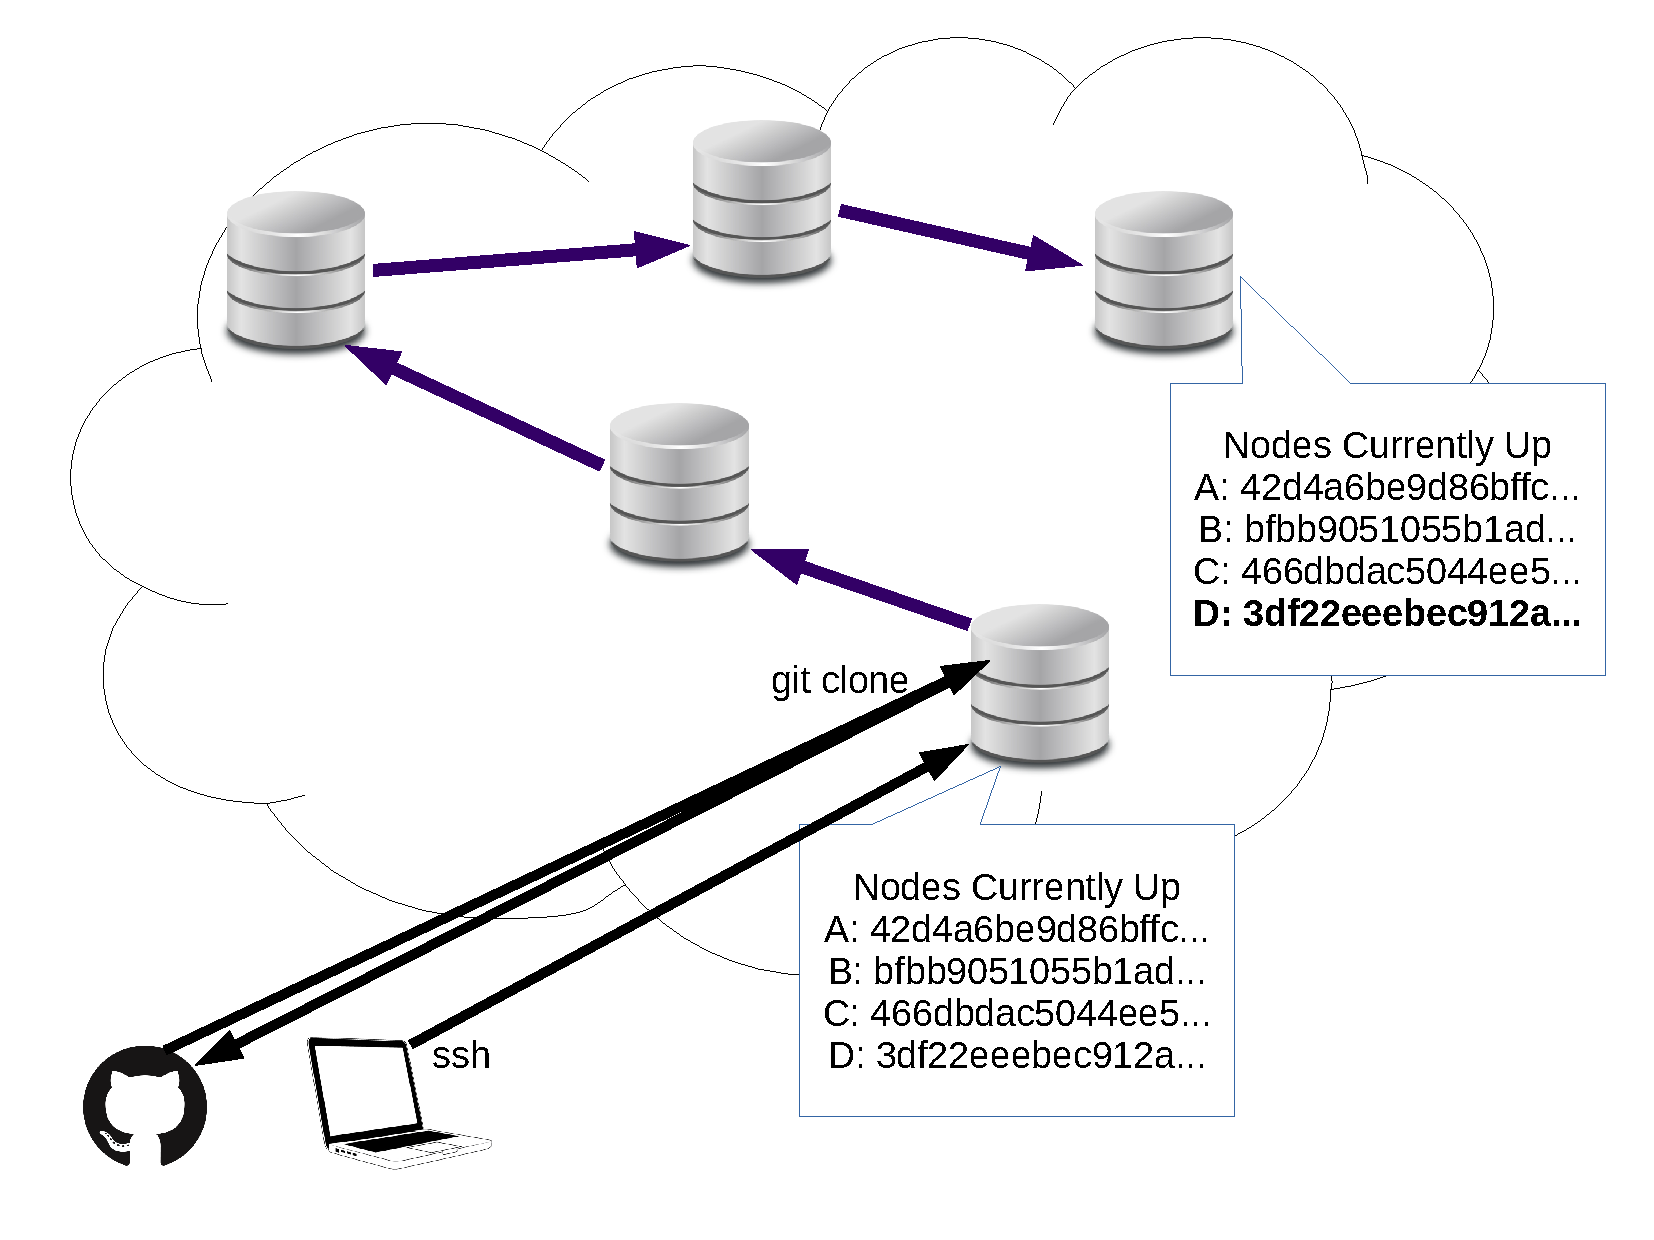
\includegraphics[scale=0.3]{figs/addingaNode.pdf}
    \\
    \small{Adding a node to the network consists of several steps. First, one needs to either obtain a VPS instance or
    server space elsewhere. Secondly, one must ssh in and `git clone' our node repo, then run an install script and
    ensure firewall settings allow inbound and outbound TCP connections from all nodes on the Up List. As load balancing
    occurs, the full amount of storage offered through the new node will be utilized -- it may take a few days.}
    \\
\end{center}

Again let's reiterate how we are different from the projects in our related works section

Describe user experience stuff

\begin{center}
    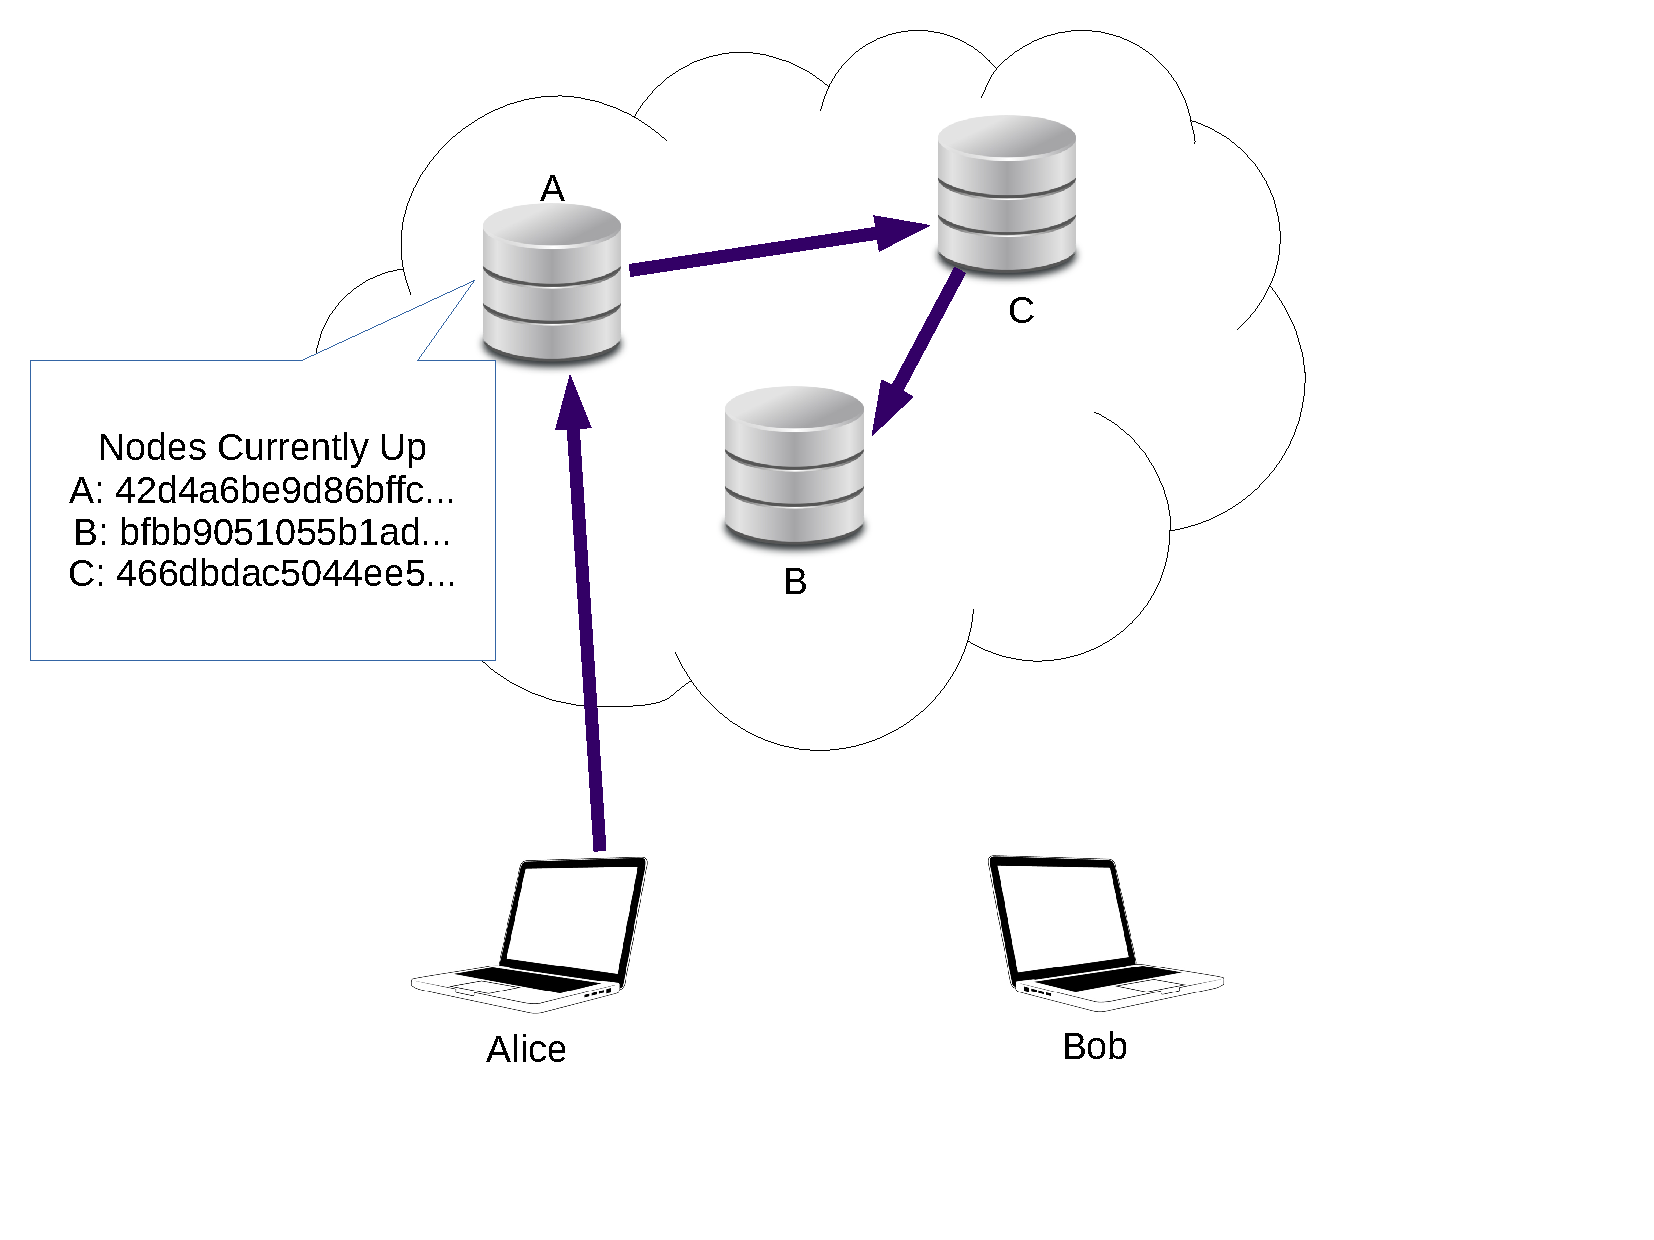
\includegraphics[scale=0.35]{figs/upload.pdf}
    \\
    \small{Uploading to the service is as simple as drag-and-drop. Within Alice's client application, the ``dropped" file
    is encrypted, and the encrypted version of the file is hashed. The encrypted file is then broken up into chunks and
    transported via PUT requests to multiple entry point nodes in the data store via several circuits.
    Each circuit constructed from Alice to
    the data store should have multiple data chunks from different parts of the file or set of files sent over it in random
    order.}
    \\
\end{center}

\begin{center}
    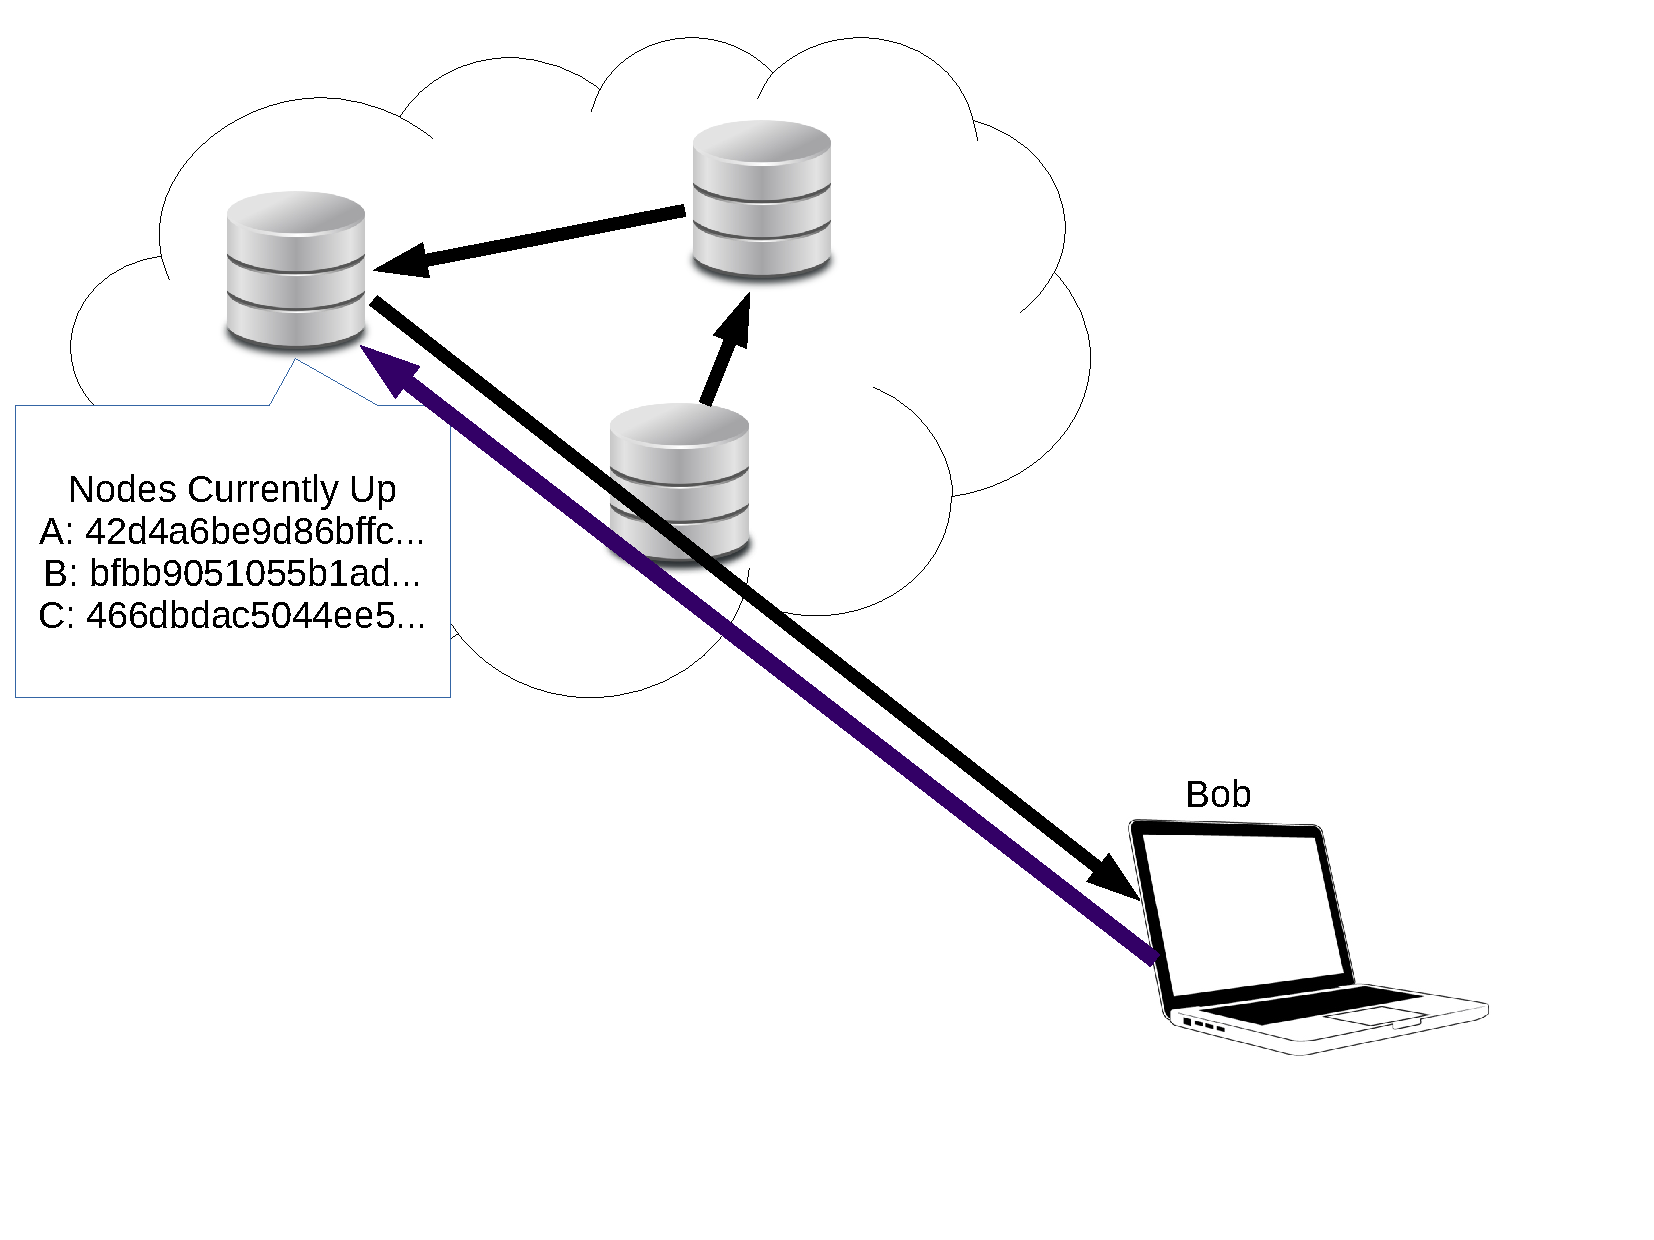
\includegraphics[scale=0.35]{figs/download.pdf}
    \\
    \small{Downloading from the service is equally user-friendly. A GET request is issued on the file's hash, and as multiple parts
    of the file trickle in, any missing pieces can be reconstructed via secret-sharing. As pieces either are pulled from the data store
    or reconstructed, a rolling checksum against the file's hash is performed, ensuring malicious add-ons are not incorporated into the
    reconstructed encrypted file. }
    \\
\end{center}

Bamboo underlies a nosqlesque key-value store application unrolled on each vps contribution

Updates to vps nodes are centrally controlled using github and implemented by users doing `git clone' and 'make'

We might also do something with puppet and/or rsync if needed but likely not

Everything is implemented on planetlab for now but more nodes will be added on actual vpses once we iron out those pesky details

Now for some stats and facts about our performance and possibly even our performance with routing algorithms other than Chord-FRT

Lastly we'll talk about what our next steps are

